\documentclass{beamer}
 
\usepackage[utf8]{inputenc}
\usepackage[brazil]{babel} % pacote portugues brasileiro
\usepackage{textpos}
\usepackage{hyperref}
\definecolor{blue(pigment)}{rgb}{0.2, 0.2, 0.6}
\hypersetup{
    colorlinks=true,
    linkcolor=blue(pigment),
    filecolor=magenta,      
    urlcolor=cyan,
}
\usetheme{Montpellier}
\usecolortheme{rose}
% \graphicspath{{../../../2021-1/DesWebBasico/aulas/fig/}}
% Layout da pagina
\hypersetup{pdfpagelayout=SinglePage}
 
%Information to be included in the title page:
\title[Introdução ao PHP]{Sintaxe básica da linguagem PHP}
 \subtitle{Disciplina: Desenvolvimento de Sistemas com PHP}
\author{Juliana C. Silva}
\institute{Universidade Positivo}

\definecolor{UniGray}{RGB}{192,192,192}
\definecolor{nGray}{RGB}{220,220,220}

\setbeamercolor{block title}{use=structure,bg=UniGray}
\setbeamercolor{block body}{use=structure,bg=nGray}
\setbeamersize{text margin left=25pt,text margin right=25pt}
\setbeamertemplate{navigation symbols}{}%remove navigation symbols
 
% Configurando layout para mostrar codigos C++
\usepackage{listings}
\lstset{
  language=PHP,
  basicstyle=\ttfamily\small, 
  keywordstyle=\color{blue}, 
  stringstyle=\color{red}, 
  commentstyle=\color{red}, 
  extendedchars=true, 
  showspaces=false, 
  showstringspaces=false, 
  numbers=left,
  numberstyle=\tiny,
  breaklines=true, 
  backgroundcolor=\color{green!10},
  breakautoindent=true, 
  captionpos=b,
  xleftmargin=0pt,
}

\begin{document}
%-----------------------------------------------------------------------
\frame{\titlepage}
 
\addtobeamertemplate{frametitle}{}{%
\begin{textblock*}{100mm}(.8\textwidth,-1.45cm)
%\includegraphics[height=0.8cm,width=2.5cm]{logo_unicesumar.png}
\end{textblock*}
}
%------------------------------------------------------------------------
\begin{frame}
\frametitle{Roteiro} 
\tableofcontents 
\end{frame}
%-----------------------------------------------------------------------
\section{Entendendo PHP}
\begin{frame}{O que é PHP?}
\begin{block}{PHP difinição}
O PHP (um acrônimo recursivo para PHP: Hypertext Preprocessor) é uma linguagem de script open source de uso geral, muito utilizada, e especialmente adequada para o desenvolvimento web e que pode ser embutida dentro do HTML.\\
\tiny{\textbf{Fonte:} \cite{achout2022php}}
\end{block}
\end{frame}
%-----------------------------------------------------------------------
\begin{frame}{Exemplo PHP}
\begin{center}
		  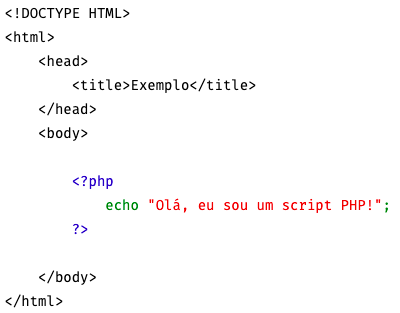
\includegraphics[height=0.65\paperheight]{fig/aula4/php_aula4_1.png} \\
		  \tiny Código PHP - Fonte: \cite{achout2022php}.
	  \end{center}
    
\end{frame}
%-----------------------------------------------------------------------
\begin{frame}{O que o PHP pode fazer?}

Qualquer coisa. O PHP é focado principalmente nos scripts do lado do servidor, portanto, você pode fazer qualquer coisa que outro programa CGI pode fazer, como:
\begin{itemize}
    \item Coletar dados de formulários;
    \item Gerar páginas com conteúdo dinâmico;
    \item Enviar e receber cookies.
\end{itemize}
 Mas o PHP pode fazer muito mais...
\end{frame}
%-----------------------------------------------------------------------
\begin{frame}{Áreas do PHP}

Existem três áreas principais onde os scripts PHP são usados:
\begin{itemize}
    \item \textbf{Scripts no lado do servidor (server-side)}: 
    \item \textbf{Scripts de linha de comando};
    \item \textbf{Escrever aplicações desktop}.
\end{itemize}
\end{frame}
%-----------------------------------------------------------------------
\begin{frame}{Áreas do PHP}
\begin{block}{Server side}
Este é o mais tradicional e principal campo de atuação do PHP. Você precisa de três coisas para isto funcionar: 
\begin{enumerate}
    \item O interpretador do PHP (CGI ou módulo do servidor);
    \item Um servidor web;
    \item Um navegador web.
\end{enumerate} 
Você precisa rodar o servidor web conectado a uma \underline{instalação do PHP}.\\ 
Você pode acessar os resultados de seu programa PHP com um navegador web, visualizando a página PHP através do servidor web. \\
Tudo isso pode rodar na sua máquina pessoal se você estiver apenas experimentando programar com o PHP. 

\end{block}
    \tiny Fonte: \cite{achout2022php}.
\end{frame}

%-----------------------------------------------------------------------
\begin{frame}{Áreas do PHP}
\begin{block}{Scripts de linha de comando}
Você pode fazer um script PHP para executá-lo sem um servidor ou navegador. A única coisa necessária é o \underline{interpretador PHP}. \\
Esse tipo de uso é ideal para script executados usando o cron (Unix, Linux) ou o prompt de comando (\textbf{cmd} no Windows). Esses scripts podem ser usados também para rotinas de processamento de texto simples. 
\end{block}
\tiny Fonte: \cite{achout2022php}.
    
\end{frame}
%-----------------------------------------------------------------------
\begin{frame}{Áreas do PHP}
\begin{block}{Escrever aplicações desktop}
O PHP provavelmente não é a melhor linguagem para criação de aplicações desktop com interfaces gráficas, mas se você conhece bem o PHP, e gostaria de usar alguns dos seus recursos avançados nas suas aplicações do lado do cliente, você pode usar o PHP-GTK para escrever programas assim. Você também tem a possibilidade de escrever aplicações multi-plataformas desse jeito. O PHP-GTK é uma extensão do PHP, não disponibilizada na distribuição oficial. 
\end{block}
\tiny Fonte: \cite{achout2022php}.
    
\end{frame}
%-----------------------------------------------------------------------
\section{Sintaxe PHP}
\begin{frame}{Sintaxe básica PHP}
Por se tratar de uma linguagem interpretada vovê precisará de um interpretador PHP.\\
\textbf{Utilizaremos o \textcolor{red}{Apache}, a instalação deste interpretador pode ser acessada através do programa XAMPP.}\\
\begin{block}{Como executar um código PHP??}
Diferentemente do HTML, que utiliza apenas o navegador, o PHP precisa ser acessado de maneira lógica, e não física, através de um "domínio virtual", gerado pelo servidor web utilizado.\\
\vspace{0.5cm}

\end{block}
    
\end{frame}
%-----------------------------------------------------------------------
\section{Executar um script PHP}
\begin{frame}{Executando uma aplicação PHP}
Para executar um script PHP:
\begin{enumerate}
    \item Inicia a aplicação XAMPP;
    \item No XAMPP, incie servidor Web Apache;
    \item Abra seu navegador Web;
    \item Acesse \textcolor{red}{http://192.168.64.2/sua\_pasta} \footnote{IP definido pelo XAMPP versão 8.0.9-0};
\end{enumerate}

Para ver e editar os arquivos PHP, estes deverão estar localizados $C:\diagdown XAMPP\diagdown htdocs$.\\
\vspace{0.5cm}
\textcolor{gray}{Os passos acima devem ser realizados antes de acessar os arquivos PHP, já que o Apache instalado via XAMPP faz a montagem da pasta htdocs quando é inicializado.}

\end{frame}

%-----------------------------------------------------------------------
\section{Olá mundo com PHP}
\begin{frame}{Executando sua primeira aplicação PHP}
Para executar um script PHP:
\begin{enumerate}
    \item Faça os passos enumerados 1 e 2 do slide anterior;
    \item Na pasta $C:\diagdown XAMPP\diagdown htdocs$ crie uma pasta chamada \textbf{aulas}; 
    \item Dentro da pasta \textbf{aulas} crie um arquivo chamado \textit{exemplo1.php};
\end{enumerate}
\begin{center}
    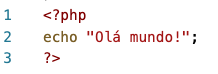
\includegraphics[height=0.2\paperheight]{fig/aula4/php_aula4_2.png}\\
    \tiny{Código PHP no arquivo exemplo1.php}
\end{center}
No navegador Web, acesse \textcolor{red}{http://192.168.64.2/aulas/exemplo1.php}.
\end{frame}
%--------------------------------------------------------------------------
\section{Tipos de dados PHP}
\begin{frame}{Variáveis}
PHP é uma linguagem \textbf{Não "tipada"}, ou seja, não é necessário determinar o tipo da variável para declara-la.\\
\begin{block}{Declaração de variáveis}
\begin{center}
		\lstinputlisting[linerange={3-4}]{fig/aula4/olamundo.php}
		\tiny Variáveis nome (texto) e idade (numérica).
	\end{center}
\end{block}
\end{frame}
%--------------------------------------------------------------------------
\begin{frame}{Variáveis}
\begin{block}{Exibindo variáveis}
\begin{center}
		\lstinputlisting[linerange={14-14}]{fig/aula4/olamundo.php}
		\tiny Imprimindo variáveis com aspas simples e operador de concatenação '.'.\\
		\lstinputlisting[linerange={15-15}]{fig/aula4/olamundo.php}
		\tiny Imprimindo variáveis com aspas duplas sem a necessidade de operador de concatenação.\\
	\end{center}
\end{block}

	\begin{center}
		  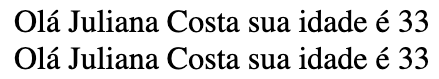
\includegraphics[height=0.1\paperheight]{fig/aula4/php_aula4_3.png} \\
		  \tiny Saída no navegador.
	  \end{center}
	  
\end{frame}
%--------------------------------------------------------------------------
\begin{frame}{Comentários PHP}
\begin{block}{Comentários}
\begin{center}
		\lstinputlisting[linerange={6-6}]{fig/aula4/olamundo.php}
		\tiny Comentar uma linha.\\
		\lstinputlisting[linerange={7-10}]{fig/aula4/olamundo.php}
		\tiny Comentar várias linhas.\\
	\end{center}
\end{block}
\end{frame}

%--------------------------------------------------------------------------
\section{Operadores}
\begin{frame}{Operadores matemáticos}
Soma
\begin{center}
		\lstinputlisting[linerange={18-19}]{fig/aula4/olamundo.php}
		\tiny Soma.\\
	\end{center}


Subtração
\begin{center}
		\lstinputlisting[linerange={21-22}]{fig/aula4/olamundo.php}
		\tiny Subtração.\\
	\end{center}
	
Multiplicação
\begin{center}
		\lstinputlisting[linerange={24-25}]{fig/aula4/olamundo.php}
		\tiny Multiplicação.\\
\end{center}

\end{frame}

%--------------------------------------------------------------------------
\begin{frame}{Operadores matemáticos [2]}
Divisão
\begin{center}
		\lstinputlisting[linerange={27-28}]{fig/aula4/olamundo.php}
		\tiny Divisão.\\
	\end{center}


Potenciação
\begin{center}
		\lstinputlisting[linerange={30-31}]{fig/aula4/olamundo.php}
		\tiny Potenciação.\\
	\end{center}
Resto da divisão
\begin{center}
		\lstinputlisting[linerange={33-34}]{fig/aula4/olamundo.php}
		\tiny Resto da divisão.\\
\end{center}
\end{frame}
%--------------------------------------------------------------------------
\section{Utilidades!}
\begin{frame}{Dica!}
Como saber o tipo da variável?
\begin{center}
		\lstinputlisting[linerange={38-38}]{fig/aula4/olamundo.php}
		\tiny Função nativa do PHP para identificar o tipo da variável.\\
	\end{center}


Como associar um valor booleano a uma variável?
\begin{center}
		\lstinputlisting[linerange={36-36}]{fig/aula4/olamundo.php}
		\tiny Declarando e inicializando uma varável booleana.\\
	\end{center}
\end{frame}
%-----------------------------------------------------------------------
\section{Referências}
\begin{frame}{Referências}%[allowframebreaks]
\frametitle{Referências}
\small
\begin{center}
\tiny
\bibliographystyle{apalike}
\bibliography{ref_aula}
\end{center}
\end{frame}
%-----------------------------------------------------------------------
 
\end{document}
